\section{Description Of The Algorithm}
%Introduce the system model by explaining the FFAST (dual problem - IFFT) architecture and then describe the decoding algorithm - peeling (multiple matches case) and Product code approach (only one exact match case).      
In this section we describe our algorithm, with sample and time complexities that are sub-linear in $N$, to find the locations $\underline{\tau} = (\tau_1, \tau_2, \cdots \tau_L)$ in the string $\xv$, where the string (query) $\yv$ matches. This is achieved by computing the cross-correlation $\rv$ of $\xv$ and $\yv$, defined in Eqn.~\eqref{Eqn:DefCrossCorrelation}, and finding the positions where there is a significant peak. 

The main idea here is that $\RXYv$ is sparse (upto some noise) with dominant peaks at $L$ positions ($\tau$) where the strings match, and noise components at $N-L$ positions where the strings do not match. Consider the case of exact matching,
\begin{equation} \label{eqn:RXY_sparse}
r[m] \ = \left\{
\begin{array}{ll}
  &M , \ \ \  \text{if} \ m \in \mathcal{T} \\
  & n_m , \ \ \ m \in [N]-\mathcal{T}
\end{array} 
\right.  
\end{equation}
where, $ \mathcal{T}:=\{\tau_1, \tau_2, \cdots, \tau_L\}$,
% $M-K \leq v_m \leq M $ is the signal component and
 $n_m$ is the noise component that is induced due to correlation of two i.i.d. sequence of random variables each taking values from $\mathcal{A} := \{+1,-1\}$. The $\rv$ can also be computed as shown below:
\begin{equation}\label{eqn:Rxy_fourier}
  \rv = \underset{\text{ \RNum{1} } } {\mathcal{F}_{N}^{-1}} \ \{ \underset{\text{ \RNum{2} } }{  \mathcal{F}_{N}\{\xv\}}  \odot \ \underset{\text{ \RNum{3} } }{ \mathcal{F}_{N}\{\yv'\}}  \} 
\end{equation} 
where $\mathcal{F}_{N}\{ \cdot \}$ and $\mathcal{F}_{N}^{-1}\{ \cdot \}$ refers to $N$-point discrete Fourier transform and its inverse respectively, $\odot$ is the point-wise multiplication operation and ${ y'[n]} = { y^{*}[-n]}$. Fig.~\ref{fig:notional} presents a notional diagram of our Algorithm.

 As evident from Equation~\ref{eqn:Rxy_fourier}, our algorithm for computing $R_{XY}$ consists of three stages:

\begin{figure}[h!]
	\begin{center}
		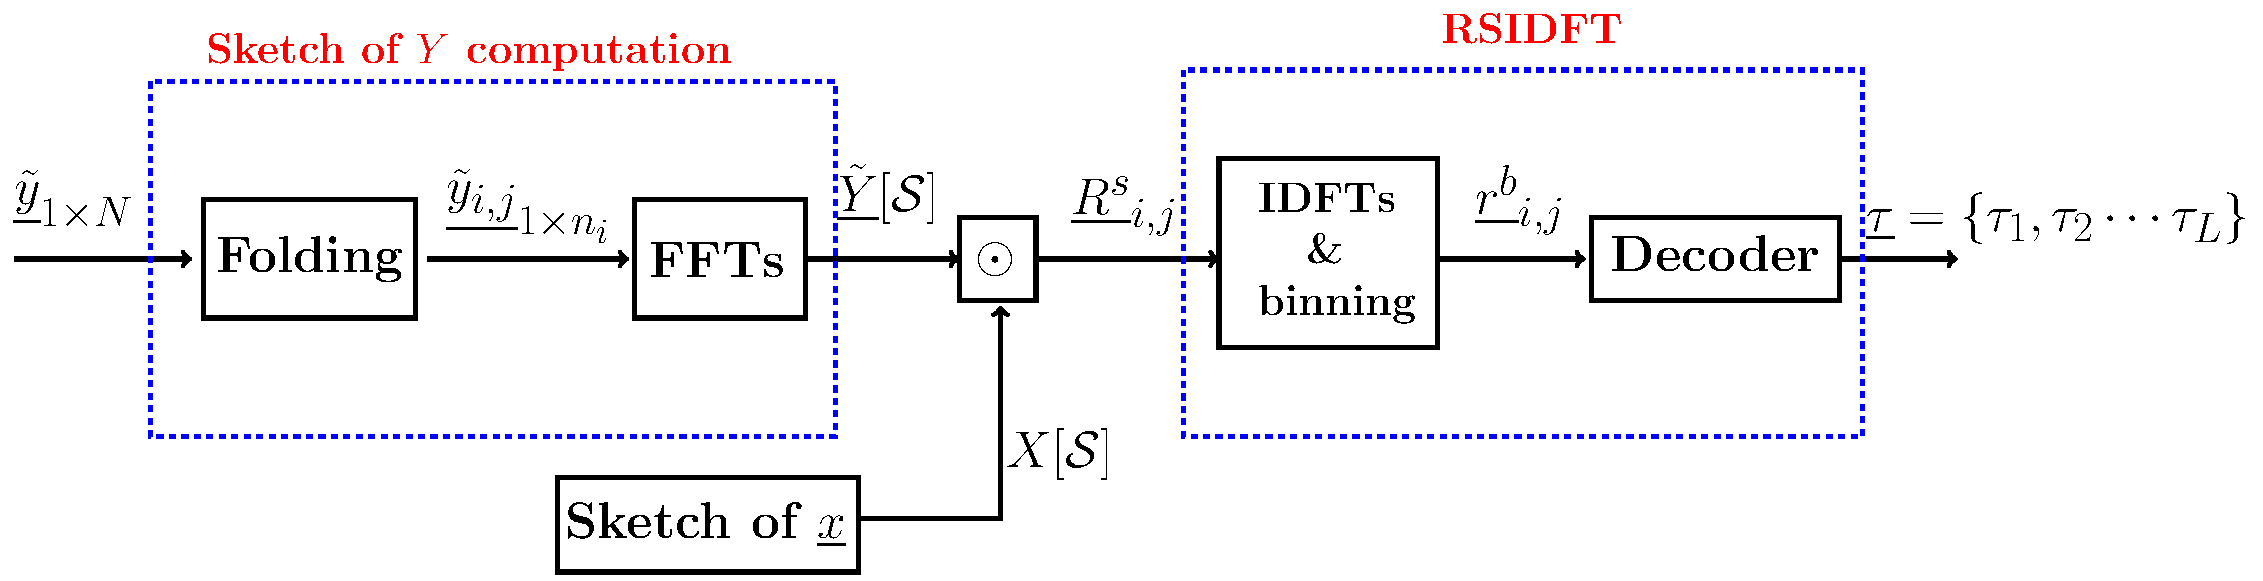
\includegraphics[height=3cm]{Figures/notional_diag} 
	\end{center}	   
	\caption{}\label{fig:notional}
	\vspace{5 pt}
\end{figure}

\begin{enumerate}
\item[\RNum{1}] \textit{Computing sparse $\mathcal{F}^{-1}$}:	

Since $\rv$ is sparse, we use a Robust Sparse Inverse  Discrete Fourier Transform(RSIDFT) framework to compute the $L$-sparse coefficients. The architecture of RSIDFT is similar to FFAST proposed in \cite{pawar2014robust}, but the decoding algorithm has some key modifications to handle the noise model induced in this problem.
 
\subsection{RSIDFT Framework} 	
\label{subsec:RSIDFT}	
	  Let $ \Rv  =  \Xv \odot \Yv'$ be the FFT of the cross-correlation of $\xv$ and $\yv$. We will see in Sec.~\ref{subsec:skteches} how do we compute the required samples of $\Xv$ and $\Yv$ but for this section we will assume that $\Xv$ and $\Yv$ are available and the required samples of $\Rv$ is computed and input to RSIDFT framework. The RSIDFT framework computes the $L$ dominant coefficients of $\rv$ by using only a sub-sampled version of $\Rv$.\\
	  	  
Consider the RSIDFT framework shown in Figure~\ref{fig:rsidft}. The framework consists of {\it $d$-stages}, each with a different sub-sampling factor $f_i$ computed as following. Let $N = P_1 \times P_2 \times \cdots P_d$ be the prime factorization of $N$, the length of the signal $\xv$. For a given $\alpha$, we choose distinct $f_i = \prod P_j$, $i \in [d]$ such that $f_i \approxeq N^{\alpha} $. In each stage, there are {\it $B$ branches} with shifts from $\underline{s}\ = [s_1, s_2, \cdots s_B] $, where $s_1 =0$ in the first branch and the rest chosen randomly from $[N^{\alpha}]$. We can also carefully choose the shifts to satisfy mutual coherence property and restricted isometric property described in the analysis section.\\
	   
	 \begin{figure}[h!]
	 	\begin{center}
	 		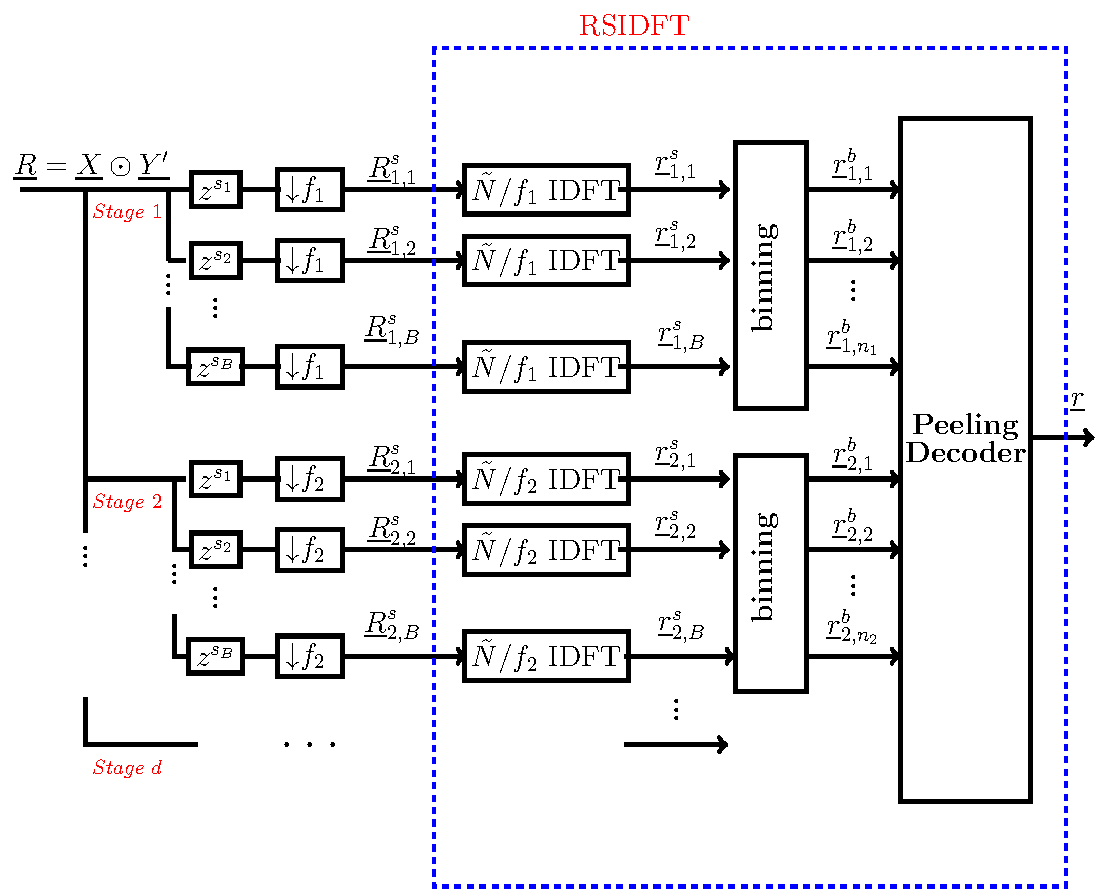
\includegraphics[height=7cm]{Figures/FFAST_Robust} 
	 	\end{center}	   
	 	\caption{ RSIDFT Framework to compute inverse Fourier Transform of a signal $\Rv$ that is sparse in time domain. }\label{fig:rsidft}
	\vspace{5 pt}
	 \end{figure}
	 	
	 Given the input $\Rv$, in branch $j$ of $i^{\text{th}}$ stage or referred to as \textit{branch $(i,j)$} for convenience, RSIDFT sub-samples the signal $\Rv$ at
\begin{align*}
	 \mathcal{S}_{i,j} \coleq \{s_j,\ s_j + f_i,\ s_j + 2f_i,\ \cdots s_j + n_i f_i\},
\end{align*}
where $n_i\coleq \lfloor{\frac{N}{f_i} }\rfloor$ to obtain $\Rv^{s}_{i,j}=\Rv[\mc{S}_{i,j}]$. The sub-sampling operation is followed by a $n_i$-point IDFT in each branch of stage $i$ to obtain $ \rv^{s}_{i,j}$. Notice that $ \rv^{s}_{i,j}$ is an aliased version of $\rv$ due to the property that sub-sampling in Fourier domain is equivalent to aliasing in time domain.\\

	 Let $\rv^{b}_{i,p_i}$ be the  vector of observations that is formed by combining all $p_i^{\text{th}}$ coefficients of $\rv^{s}_{i,j}$ (belonging to stage $i$) together as a vector, where $1 \leq p_i \leq n_i$, i.e.
\[
	  \rv^{b}_{i,p_i} = \begin{bmatrix}
	 r^{s}_{i,1}[p_i] \\
	 r^{s}_{i,2}[p_i] \\
	 \vdots\\
	 r^{s}_{i,B}[p_i]
	 \end{bmatrix}  
\]

\begin{figure}[h!]
	\begin{center}
		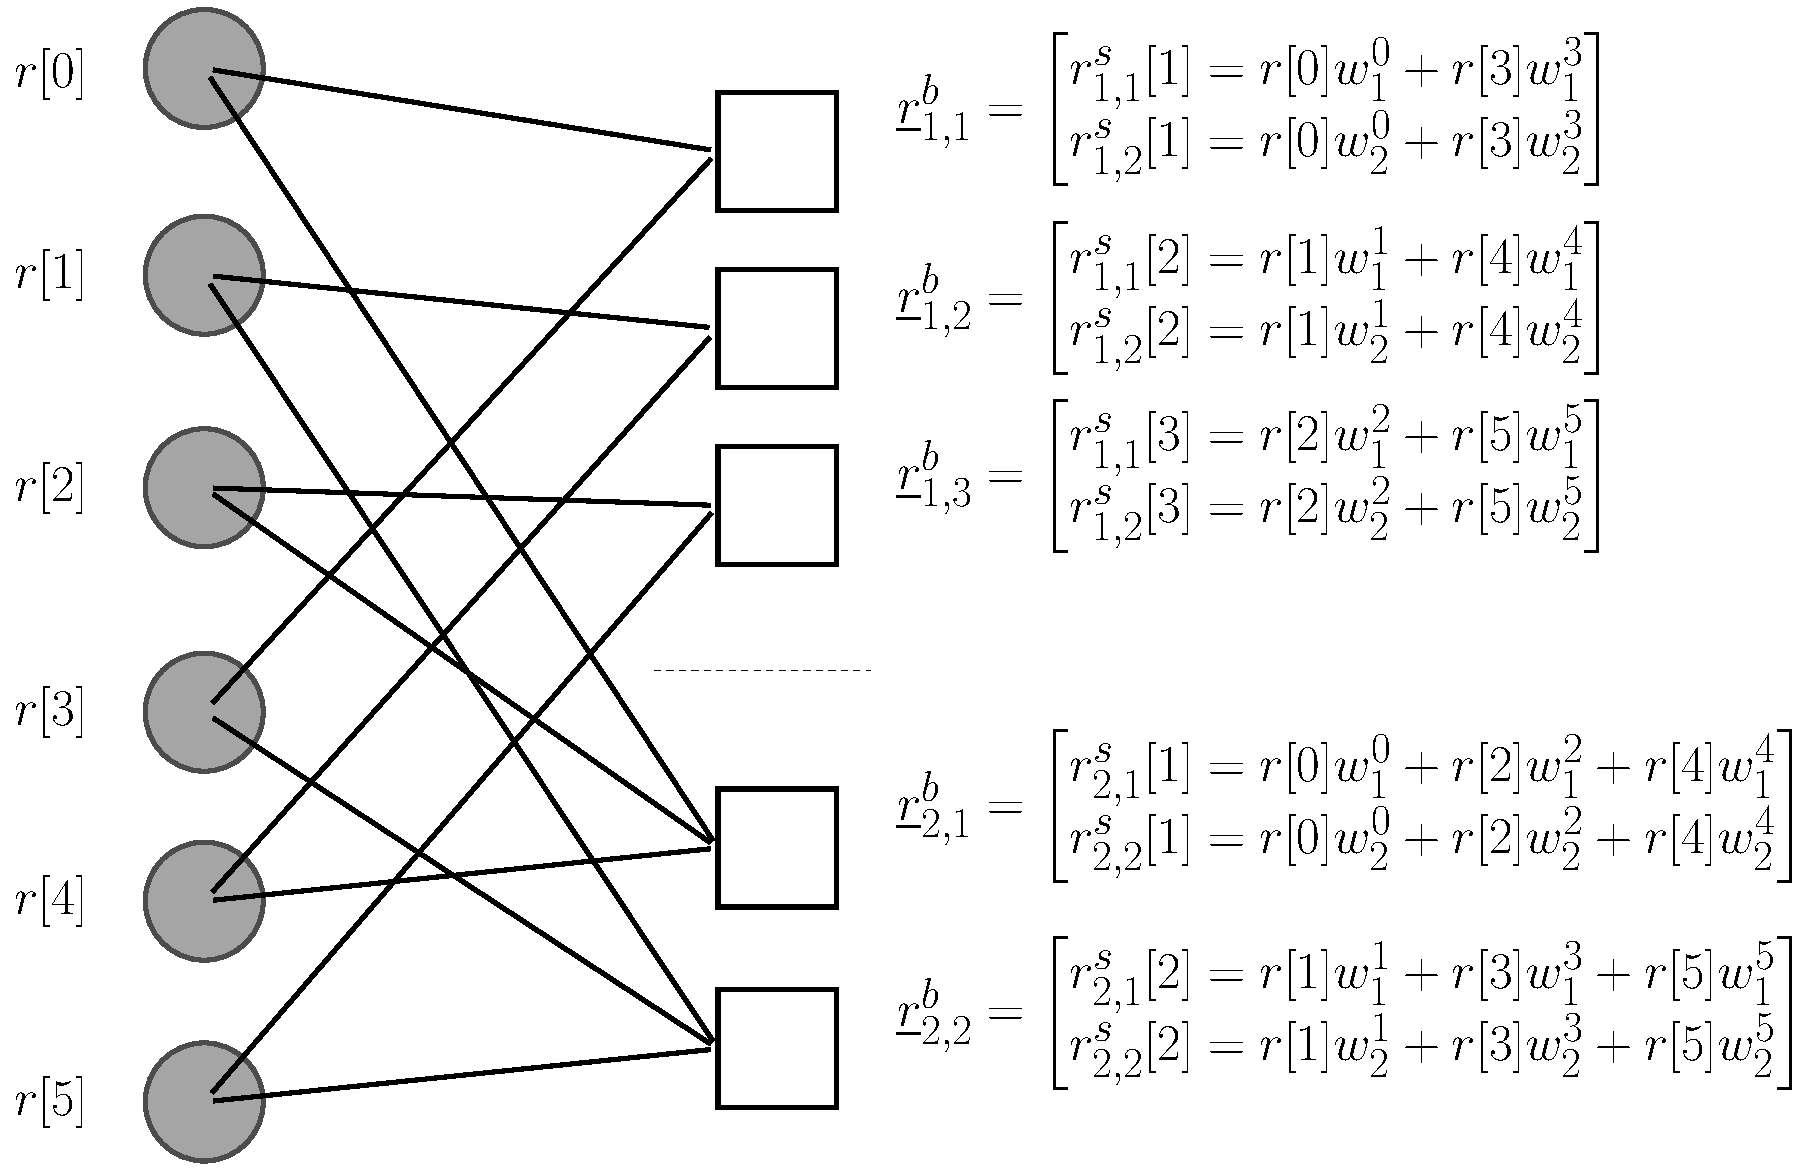
\includegraphics[height=7cm]{Figures/Factorgraph} 
	\end{center}	   
	\caption{Example of a Tanner graph formed in a RSIDFT framework with system parameters being $d=2$, $B=2$, $N=6$, $f_1 = 2$ and $f_2=3$. The variable nodes (colored gray circles) represent the cross-correlation vector $\rv$ and the bin nodes (uncolored white boxes) represent the binned observation vector $\rv_{i,p_i}^b$. Figure also illustrates the relationship between $\rv_{i,p_i}^b$ and $\rv$.}\label{fig:factorgraph}
	\vspace{5 pt}
\end{figure}

In Fig.~\ref{fig:factorgraph} we represent the relation between $\rv$ and $\tilde{\rv}^{b}\coleq[\rv^{b}_{1,1},\rv^{b}_{1,2},\ldots,\rv^{b}_{1,n_1},\ldots, \rv^{b}_{2,1},\ldots,\rv^{b}_{2,n_2},\ldots, \rv^{b}_{B,1},\ldots,\rv^{b}_{B,n_B}]$, aliased versions of the cross-correlation vector $\rv$ concatenated together, via a Tanner graph. We refer to $\tilde{\rv}^{b}$ as sensing signal. The nodes on the left, which we refer to as {\it variable nodes}, represent the $N$ elements of vector $\rv$. And similarly the nodes on the right, which we refer to as {\it bin nodes}, represent the $\sum_{i\leq B} n_i$ sub-sensing signals. We will now describe the decoding algorithm which takes the sensing signal $\tilde{\rv}^b$ as input and estimates the $L$-sparse $\rv$.	 

\subsection{Decoder}		
	%\textcolor[rgb]{0,0.3,0.7}{Maybe remove Each coefficient of $\rv^{b}_{i,p_i}$ is a bin that has $N^{\alpha}$ coefficients from $\RXYv$ hashed into it. This can be seen using a Tanner graph with $\RXYv$ as the left nodes (bit nodes) and the aliased coefficients $\rv^{b}_{i,p_i}$ as the right nodes (check-nodes).}
	
	Observe from the Tanner graph that the degree of each bit node is $d$ and that of each bin node is approximately $N^{\alpha}$. 
We refer to a bin node as {\it zero-ton} (or $\mc{H}_z$) if the number of variable nodes with significant amplitude connected to the bin node is zero. The {\it singleton ($\mc{H}_s$), double-ton ($\mathcal{H}_d$) and multi-ton ($\mc{H}_m$)} bin nodes are defined similarly where the number of significant variable nodes connected are one, two and greater than two, respectively. The peeling decoder has the following three steps in the decoding process.\\

\begin{itemize}
\itemsep4pt
\item \textit{Bin Identification}: In this step a bin node is classified as a zero-ton or a singleton or a multi-ton. At bin $(i,j)$ the classification is done based on  comparing the first observation $r^{b}_{i,j}[1]$, which corresponds to zero shift, with a predefined threshold. The threshold is set differently for Exact Matching and Approximate Matching cases. Let the value of $r^{b}_{i,j}[1]$ be $z$, then the classification rules can be written as follows:\\
{\bf Exact Matching:} 
$$
\mc{H}(i,j)=
\begin{cases}
\mc{H}_z &  		z/M < 0.5 \\
\mc{H}_s &	 0.5 \leq z/M \leq 1.5 \\ 
\mc{H}_d \text{ or } \mc{H}_m  &       z/M > 1.5
\end{cases}
$$
{\bf Approximate Matching:} 
$$
\mc{H}(i,j)=
\begin{cases}
\mc{H}_z &  	 z/M < \gamma_1\\
\mc{H}_s &	  \gamma_1 < z/M < \gamma_2  \\
\mc{H}_d  &    \gamma_2  < z/M <  \gamma_3\\ 
\mc{H}_m &      z/M > \gamma_3\\
\end{cases}
$$ 
where $(\gamma_1,\gamma_2,\gamma_3)=(\frac{(1-3\eta/2)}{2},\frac{(1-\eta/2)3}{2},\frac{(5-3\eta)}{2})$.
			   
\item \textit{Position Identification}: If a bin node $(i,j)$ is classified as a singleton, we need to identify the position of the significant non-zero variable node connected to it. This is done by correlating the observation vector $\rv^{b}_{i,j}$ with each column of $S = [\underline{s_1} \ \underline{s_2} \cdots \underline{s_A}]$ and then picking the column index, $p'$ that produced the maximum correlation value.
\begin{align*}
 p' = \underset{l}{\argmax}\  \underline{s}^T_l ~ \rv^{b}_{ij}
\end{align*} 
Given that a check-node is classified as a Single-ton, we need to identify the position of the non-zero coefficient  hashed into it. This is done by correlating the observation vector $\underline{z^{b}_{i,p_i}}$ with each column $\underline{g_l}$ of  $G = [\underline{g_1} \ \underline{g_2} \cdots \underline{g_A}]$, where $\underline{g_l} =\begin{bmatrix}
			 w_1^{l}, ~ w_2^{l}, ~ \cdots\, ~ w_B^{l}
			 \end{bmatrix}^{T}$ with $w_k = e^{j \frac{2\pi s_k}{N}}$,  and then picking the column index  $p'$ that produced the maximum value.
\[ p' = \underset{l}{\argmax}\  \underline{s^T_l} ~ \underline{z^{b}_{i,p_i}}\]
			 
			 \item \textit{Peeling Process: } Although the idea behind the peeling process is same for Exact Matching and the Approximate Matching scenarios, there are some minor differences in their implementation. The main idea in this peeling based decoder is to find a singleton bin, identify the variable node connected to the bin and remove it's contribution from all the bin nodes connected to this variable node.\\

\begin{algorithm}
\caption{Peeling based recovery algorithm}
\label{Algo:decoder}
\begin{algorithmic}
\While {$\exists i\in[M_1]: \mc{H}_i=\mc{H}_Z ~\text{or } \mc{H}_S $, }
\If {$\mc{H}_i=\mc{H}_Z$}
    \State Remove the bin $i$\\
   \hspace{2ex} Assign $0$ to all the variables connected
\ElsIf {$\mc{H}_i=\mc{H}_S(k,x[k])$}   
   \hspace{4ex} Assign $x[k]$ to $k^{\text{th}}$ variable in bin $i$\\
  \hspace{2ex} Subtract $x[k]\mb{s}_k$ from connected $\mb{y}_i$  \\
  \hspace{2ex} Remove the bin and all variables connected
\EndIf
\EndWhile
\end{algorithmic}
\end{algorithm}


{\bf Exact Matching:} Here we remove the identified Singleton's contribution from all the check-nodes it participates in.			  \\
{\bf Approximate Matching:} Here we only remove the identified singleton's contribution from a double-ton and do not alter multi-tons whose $degree > 2$.
\end{itemize} 
		 
 We exploit this property of sparsity to compute $\RXYv$ by using only a subset of samples from $\Xv = \mathcal{F}\{\xv\} $ and $\Yv' = \mathcal{F}\{\yv'\} $, each sampled at positions $l \in \mathcal{S}$, where $\mathcal{S} = \mathcal{S}_{1,1} \cup \mathcal{S}_{1,2} \cup \cdots \cup \mathcal{S}_{i,j} \cup  \mathcal{S}_{d,B} \subset \{ 0,1,\cdots ,N-1 \}$ and $\mathcal{S}_{i,j}$, $1 \leq i \leq d $ and  $1 \leq j \leq B $ are disjoint sets of size $|\mathcal{S}_{i,j}| \approxeq N^{1-\alpha}$ with periodic sample points from $[N]$ given by 
 
 \begin{equation}
 \label{eqn:sampling_sets}\mathcal{S}_{i,j} = \{s_j,\ s_j + f_i,\ s_j + 2f_i,\ \cdots s_j + \lfloor{\frac{N}{f_i} }\rfloor f_i \}
 \end{equation}
   where $s_j$'s and $f_i$'s are constants chosen based on the requirements from Robust Sparse Inverse Fourier Transform (RSIDFT) framework described in Section~\ref{subsec:RSIDFT}.

\subsection{Sketches of $\Xv$ and $\Yv$} 
\label{subsec:skteches}

	\item[\RNum{1}] \textit{Computing the sketch of $\xv$}: 
	 We assume that the sketch of $\xv$, \ $ \Xv[l] = \mathcal{F}\{\xv\}$ is precomputed at positions $l \in \mathcal{S}$ and stored in a database.  
	\item[\RNum{2}] \textit{Computing the sketch of $\yv$}:
	 For every new query $\yv$, $ \Yv'[l]$ is computed at $l \in \mathcal{S}$. Naively, the FFT algorithm can be used to compute this with $O(N \log N)$ complexity. Since only a subset $\mathcal{S}$ of samples from $\Yv'$ is needed, this can be done by using a folding technique described below. 
	  The idea behind this folding technique is to induce aliasing in $\yv'$ and then taking a smaller point Fourier Transform to compute the sub-sampled version $\Yv'$. Aliasing is induced by folding the signal $\yv'$ into blocks of length $N^{1-\alpha}$ and adding them. The desired sub-sampling patterns in frequency domain are induced by multiplying $\yv'$ with suitable exponentials. Let us denote the aliased versions of $\yv'$ by $\underline{y^{a}_{i,j}}'$. Then, $\underline{y^{a}_{i,j}}'$ is given by
	  \begin{equation}
	  	{y^{a}_{i,j}}'[p] = \sum \limits_{m = 0}^{\lfloor{\frac{N}{f_i}}\rfloor} y'[p + mf_i] e^{j \frac{2 \pi s_j}{N} } 
	  \end{equation}
	  Taking $\frac{N}{f_i}$ point DFT of $\underline{y^{a}_{i,j}}'$ produces $\Yv'[l]$ sub-sampled at $l \in \mathcal{S}_{i,j}$. To obtain all the samples in $\mathcal{S}$, the folding procedure needs to be carried out $dB$ times, once for each $(i,j)$ pair, where $1 \leq i \leq d $ and  $1 \leq j \leq B $.  
\end{enumerate}
